\clearpage
\phantomsection

\setcounter{chapter}{2}
\chapter[NHẬN DẠNG HỆ THỐNG SỬ DỤNG MẠNG HỌC SÂU]{Nhận dạng hệ thống sử dụng mạng học sâu}
\label{sec:ML}

Trong chương này, tác giả sẽ đề xuất một mô hình mạng học sâu ISD sử dụng cho nhận dạng hệ thống viễn thông MIMO/mMIMO. Đầu tiên, sơ lược về hai hướng tiếp cận sử dụng mạng nơ-ron học sâu sẽ được giới thiệu. Kế đến là khái niệm về kỹ thuật mở rộng sâu (Deep unfolding). Một mô hình được mở rộng sâu từ thuật toán ISD gốc là DetNet được trình bày để so sánh ở mục các kết quả mô phỏng. Tiếp đến, từ một giải thuật ISD đã được đề xuất trong~\cite{Mandloi2017}, kết hợp với cách tiếp cận mở rộng sâu tại~\cite{Liao2020}, tác giả sẽ đề xuất một mạng học sâu DNN để nhận dạng hệ thống. Các bước mô phỏng và đánh giá sẽ được đưa ra để cho thấy tiềm năng của phương pháp đề xuất và đưa ra kết luận của chương. 

\section{Giới thiệu về mạng nơ-ron học sâu và mở rộng sâu (Deep unfolding)}

Trong chương~\ref{sec:back}, các phương pháp nhận dạng hệ thống sử dụng các phương pháp ML/DL đã được chia làm ba loại, trong đó phương pháp sử dụng các mạng nơ-ron đang được quan tâm nghiên cứu. Các mạng nơ-ron sâu (DNN - Deep-neural network) đã được sử rụng rộng rãi trong các ứng dụng như xử lý tiếng nói, ngôn ngữ tự nhiên, hình ảnh, thị giác máy, trò chơi trực tuyến~\cite{Samek2021}. Mười năm trở lại đây, nhiều nghiên cứu ứng dụng các mô hình mạng DNN khác nhau cho nhận dạng hệ thống viễn thông không dây. Có thể chia các phương pháp này thành hai kiểu chính, bao gồm hướng dữ liệu (data-driven) và hướng mô hình (model-driven)~\cite{Liao2020}. Các phương pháp data-driven trực tiếp học các đặc trưng từ một tập lớn các dữ liệu (dataset) để phục vụ cho các mục đích như ước lượng kênh truyền, phản hồi CSI,~\ldots. Tuy các phương pháp data-driven được đề xuất đều cho độ chính xác cao nhưng vẫn có những thách thức khi yêu cầu số lượng mẫu rất lớn và kéo theo đó là thời gian cho việc đào tạo lâu. Các phương pháp model-driven~\cite{He2019} có thể một phần khắc phục các hạn chế này bằng việc tối ưu/đưa thêm các tham số học bằng DL vào các một hình có sẵn để kết hợp ưu điểm của data-driven và các mô hình toán học truyền thống. 

Trong các năm gần đây, kỹ thuật mở rộng sâu (Deep unfolding)~\cite{Wisdom2016} là một giải pháp tiềm năng để chuyển các giải thuật truyền thống thành các kiến trúc mạng DNN theo hướng tiếp cận model-driven. Chi tiết về mở rộng sâu tại~\cite{John2014}, chuyển đổi các phương pháp yêu cầu các vòng lặp đi lặp lại (iteractive inference) sang từng lớp của một mạng NN. Sau đó, sử dụng các giải thuật giảm độ dốc dự kiến (gradient descent), các tham số đào tạo trên các lớp được tách ra và đào tạo một cách riêng biệt. Sau $K$ lớp đào tạo tương tự như $K$ vòng lặp trong thuật toán gốc, mô hình có thể đạt được mục tiêu mong muốn. Ví dụ, DetNet~\cite{Samuel2017} là một mạng DNN dựa trên việc mở rộng sâu giải thuật `projected gradient descent'~\cite{Chen2015} cho bộ tối ưu hợp lẽ cực đại (MLE). Trong mục tiếp theo, mô hình mạng nơ-ron sâu DetNet sẽ được giới thiệu ngắn gọn và kết quả của DetNet sẽ so sánh với mạng sẽ được đề xuất.

\section{Mạng nơ-ron học sâu DetNet}

Xét hệ thống MIMO/mMIMO tương tự đã trình bày ở hình~\ref{fig:sys_model}. Tuy nhiên, thay vì mô hình hoá tín kênh truyền vô tuyến dưới dạng các bộ lọc FIR có chiều dài $M+1$, trong DNN, giả sử: (i) $T$ có thể coi là số lượng ăng-ten bên phát hoặc số lượng người dùng (user) với mỗi người dùng chỉ có một ăng-ten phát, (ii) ma trận $\mathbf{H}$ là biến đổi tuyến tính của tín hiệu truyền thành tín hiệu nhận được, (iii) $N=1$ tức mỗi ăng-ten nhận chỉ thu thập một ký hiệu tại một thời điểm, (iv) các ma trận sẽ được chuyển đổi sang dạng phần thực, ảo riêng biệt như phương trình (\ref{eq:matrixtras1}) và (\ref{eq:matrixtras2}). Biểu diễn đơn giản cho hệ thống MIMO/mMIMO như sau
\begin{equation}
    \mathbf{x} = \mathbf{H} \mathbf{s} + \mathbf{w}
\end{equation}
trong đó, $\mathbf{H} \in \mathbb{R}^{2L \times 2T}$, $\mathbf{s} \in \mathbb{R}^{2T \times 1}$, $\mathbf{w} \in \mathbb{R}^{2L \times 1}$, và $\mathbf{x} \in \mathbb{R}^{2L \times 1}$. Để tìm bộ nhận dạng cho hệ thống kể trên, định nghĩa hàm mất mát $l\left(\mathbf{s} ; \hat{\mathbf{s}}_{\boldsymbol{\theta}}(\mathbf{H}, \mathbf{x})\right)$ là khoảng cách giữa ký hiệu gốc và ký hiệu được ước lượng. Tìm giá trị $\mathbf{\theta}$ bằng cách tối thiểu hoá hàm mất mát kể trên.
\begin{equation}
\label{eq:lossf}
\min _{\boldsymbol{\theta}} \mathbb{E}\left\{l\left(\mathbf{s} ; \hat{\mathbf{s}}_{\boldsymbol{\theta}}(\mathbf{H}, \mathbf{x})\right)\right\}
\end{equation}

Giải thuật cho độ chính xác cao nhất để giải quyết (\ref{eq:lossf}) là bộ ước lượng hợp lẽ cực đại (MLE - Maximum likelihood estimator) như sau
\begin{equation}
\label{eq:mle}
\hat{\mathbf{s}}_{\boldsymbol{\theta}}(\mathbf{x}, \mathbf{H})=\arg \min _{\mathbf{s} \in \mathbb{R}^{2T}}\|\mathbf{x}-\mathbf{H} \mathbf{s}\|^2
\end{equation}
Tuy nhiên, độ phức tạp của MLE sẽ tăng theo cấp số mũ $\mathcal{O}(2^T)$ nên khó để triển khai trong các hệ mMIMO. Do vậy, DetNet được đề xuất nhằm tạo ra một kiến trúc mạng DNN đạt được tiệm cận độ chính xác với MLE. Trong nghiên cứu gốc, thay vì tạo ra một mạng nơ-ron nhằm ánh xạ trực tiếp từ $\mathbf{x}$ về $\mathbf{s}$, việc phân tách $\mathbf{x}$ thành các thành phần $\mathbf{H}, \mathbf{s},$ và $\mathbf{w}$ sẽ hiệu quả hơn.
\begin{equation}
    \mathbf{H}^\top \mathbf{x}=\mathbf{H}^\top \mathbf{H s}+\mathbf{H}^\top \mathbf{w}
\end{equation}

Kiến trúc DetNet dựa trên phương pháp giảm độ dốc dựa kiến (projected gradient descent)~\cite{Chen2015} cho việc tối ưu MLE như trên (\ref{eq:mle}). Đạo hàm riêng được tách như trên (\ref{eq:pgd}) sử dụng luật chuỗi (chain rule)~\cite{Minka2000}.
\begin{equation}
\label{eq:pgd}
    \begin{aligned}
    \hat{\mathbf{s}}_{k+1} & =\Pi\left[\hat{\mathbf{s}}_k-\left.\delta_k \frac{\partial\|\mathbf{x}-\mathbf{H} \mathbf{s}\|^2}{\partial \mathbf{s}}\right|_{\mathbf{s}=\hat{\mathbf{s}}_k}\right] \\
    & =\Pi\left[\hat{\mathbf{s}}_k-\delta_k \mathbf{H}^\top \mathbf{x}+\delta_k \mathbf{H}^\top \mathbf{H} \hat{\mathbf{s}}_k\right]
    \end{aligned}
\end{equation}
với $\mathbf{s}_k$ là giá trị ước lượng tại lớp thứ $k$, $\Pi [.]$ là một phép chiếu phi tuyến tính, và $\delta_k$ là độ dài bước (step size) của quá trình học. Kiến trúc của mạng DetNet đề xuất trong~\cite{Samuel2017} được biểu biến như trên hình~\ref{fig:detnet} và cách biểu diễn dưới dạng ma trận như sau
\allowdisplaybreaks
\begin{subequations}
\begin{alignat}{4}
    \mathbf{z}_k & =\rho\left(\mathbf{W}^1_{k}\left[\begin{array}{c}
    \mathbf{H}^\top \mathbf{x} \\
    \hat{\mathbf{s}}_k \\
    \mathbf{H}^\top \mathbf{H} \hat{\mathbf{s}}_k \\
    \mathbf{v}_k
    \end{array}\right]+\mathbf{b}^1_{k}\right) \\
    \hat{\mathbf{s}}_{k+1} & =\psi_{t_k}\left(\mathbf{W}^2_{k} \mathbf{z}_k+ \mathbf{b}^2_{k}\right) \\
    \hat{\mathbf{v}}_{k+1} & =\mathbf{W}^3_{k} \mathbf{z}_k+ 
    \mathbf{b}^3_{k} \\
    \hat{\mathbf{s}}_1 & =\mathbf{0}
\end{alignat}
\end{subequations}
trong đó, $k = 1, \ldots, K$ là số các lớp của mạng DetNet, $\rho$ là một toán tử tuyến tính như ReLu hoặc Tanh. $\psi_{t_k}$ ký hiệu cho hàm tuyến tính phân đoạn, ở các mức $t$ khác nhau, $\psi_{t_k}(s)$ được minh hoạ trên hình~\ref{fig:soft_sign} và có biểu diễn toán học như sau
\begin{equation}
    \psi_{t_k}(s)=-1+\frac{\rho\left(s + t_k \right)}{\left|t_k\right|}-\frac{\rho\left(s- t_k \right)}{\left|t_k\right|}
\end{equation}

\begin{figure}[tb]
    \centering
    \begin{tikzpicture}
        \node (B11) [field6, fill=red!10!white] at (0, 0) {$\mathbf{H}^\top \mathbf{x}$};
        \node (B21) [below=10mm of B11, field6, fill=red!10!white] {$\mathbf{v}_k$};
        \node (B31) [below=10mm of B21, field6, fill=red!10!white] {$\mathbf{s}_k$};
        \node (B41) [below=10mm of B31, field6, fill=red!10!white] {$\mathbf{H}^\top \mathbf{H}$};

        
        \node (B32) [right=10mm of B31.south east, anchor=north, circle, fill=blue!10!white, draw=black] {$\times$}; 
        \node (B22) [right=25mm of B21, circle, fill=blue!10!white, draw=black] {$\operatorname{con}$};
        \node (B33) [below=11mm of B22, circle, fill=blue!10!white, draw=black] {$\times$};
        \node (B34) [below=4mm of B33, field8, fill=green!10!white, draw=black] {$\mathbf{W}^1_{k}$};
        \node (B35) [right=7mm of B33, circle, fill=blue!10!white, draw=black] {$+$};
        \node (B36) [below=4mm of B35, field8, fill=green!10!white, draw=black] {$\mathbf{b}^1_{k}$};

        \node (B37) [circle, fill=blue!10!white, draw=black] at (70mm, -30mm) {$\rho$};
        \node (B38) [right=40mm of B33, circle, fill=blue!10!white, draw=black] {$\times$};
        \node (B39) [below=4mm of B38, field8, fill=green!10!white, draw=black] {$\mathbf{W}^2_{k}$};
        \node (B310) [right=7mm of B38, circle, fill=blue!10!white, draw=black] {$+$};
        \node (B311) [below=4mm of B310, field8, fill=green!10!white, draw=black] {$\mathbf{b}^2_{k}$};
        \node (B312) [right=7mm of B310, circle, fill=blue!10!white, draw=black] {$\Psi$};

        \node (B23) [above=24.2mm of B39, circle, fill=blue!10!white, draw=black] {$\times$};
        \node (B24) [right=7mm of B23, circle, fill=blue!10!white, draw=black] {$+$};
        \node (B25) [above=4mm of B23, field8, fill=green!10!white, draw=black] {$\mathbf{W}^3_{k}$};
        \node (B26) [above=4mm of B24, field8, fill=green!10!white, draw=black] {$\mathbf{b}^3_{k}$};

        \node (Bvk1) [right=123mm of B21, field6, fill=red!10!white] {$\mathbf{v}_{k+1}$};
        \node (Bxk1) [right=123mm of B31, field6, fill=red!10!white] {$\mathbf{s}_{k+1}$};

        \draw[arrow] (B312) -- (Bxk1);
        \draw[arrow] (B24) -- (Bvk1);
        \draw[arrow] (B310) -- (B312);
        \draw[arrow] (B38) -- (B310);
        \draw[arrow] (B23) -- (B24);
        \draw[arrow] (B25) -- (B23);
        \draw[arrow] (B26) -- (B24);
        \draw[arrow] (B311) -- (B310);
        \draw[arrow] (B39) -- (B38);
        \draw[arrow] (B33) -- (B35);
        \draw[arrow] (B36) -- (B35);
        \draw[arrow] (B34) -- (B33);
        \draw[arrow] (B22) -- (B33);

        \draw[arrow] (B21) -- (B22);
        \draw[line] (B11) -- ([yshift=-3mm]B11.south);
        \draw[arrow] ([yshift=-3mm]B11.south) -| (B22);
        \draw[line] (B31) -- ([xshift=3mm]B31.east);
        \draw[arrow] ([xshift=3mm]B31.east) |- ([yshift=-1.5mm]B22.west);
        \draw[line] (B32) -- ([xshift=3mm]B32.east);
        \draw[arrow] ([xshift=3mm]B32.east) |- ([yshift=-3mm]B22.west);

        \draw[arrow] (B31) |- ([yshift=3mm]B32);
        \draw[arrow] (B41) |- ([yshift=-3mm]B32);

        \draw[arrow] (B37) |- (B38);
        \draw[arrow] (B37) |- (B23);
        \draw[arrow] (B35) |- (B37);
        
        \draw[arrow] (B41) -- (150mm, -60mm);
        \draw[arrow] (Bvk1) -- (150mm, -20mm);
        \draw[arrow] (Bxk1) -- (150mm, -41mm);
        \draw[arrow] (B11) -- (150mm, 0mm);

        % Legends
        \node[rectangle, draw=black, dashed, fill=black!5!white, minimum width=140mm, minimum height=35mm] at (70mm, -85mm) {};

        \node (B51) [field6, fill=red!10!white] at (22mm, -78mm) {Giá trị \\đầu vào/đầu ra};

        \node (B61) [below=4mm of B51, field8, fill=green!10!white, draw=black] {Giá trị học};

        \node (B52) [right=7mm of B51, circle, fill=blue!10!white, draw=black] {$\times$};
        \draw[arrow] (B52) -- ([xshift=3mm]B52.east) node [pos=0, right=3mm] {Nhân};

        \node (B53) [below=7mm of B52, circle, fill=blue!10!white, draw=black] {$+$};
        \draw[arrow] (B53) -- ([xshift=3mm]B53.east) node [pos=0, right=3mm] {Cộng};

        \node (B54) [right=20mm of B52, circle, fill=blue!10!white, draw=black] {$\rho$};
        \draw[arrow] (B54) -- ([xshift=10mm]B54.east) node [pos=0, right=10mm, above, label={below}:{tuyến tính}] {Toán tử};

        \node (B55) [right=20mm of B53, circle, fill=blue!10!white, draw=black] {$\Psi$};
        \draw[arrow] (B55) -- ([xshift=10mm]B55.east) node [pos=0, right=11mm, above, label={below}:{phi tuyến tính}] {Toán tử};

        \node (B56) [right=28mm of B54, circle, fill=blue!10!white, draw=black] {$\operatorname{con}$};
        \draw[arrow] (B56) -- ([xshift=3mm]B56.east) node [pos=0, right=3mm] {Nối};
         
    \end{tikzpicture}
    \caption{Kiến trúc của một lớp trong mô hình mạng DetNet~\cite{Samuel2017}.}
    \label{fig:detnet}
\end{figure}

\begin{figure}[H]
    \centering
    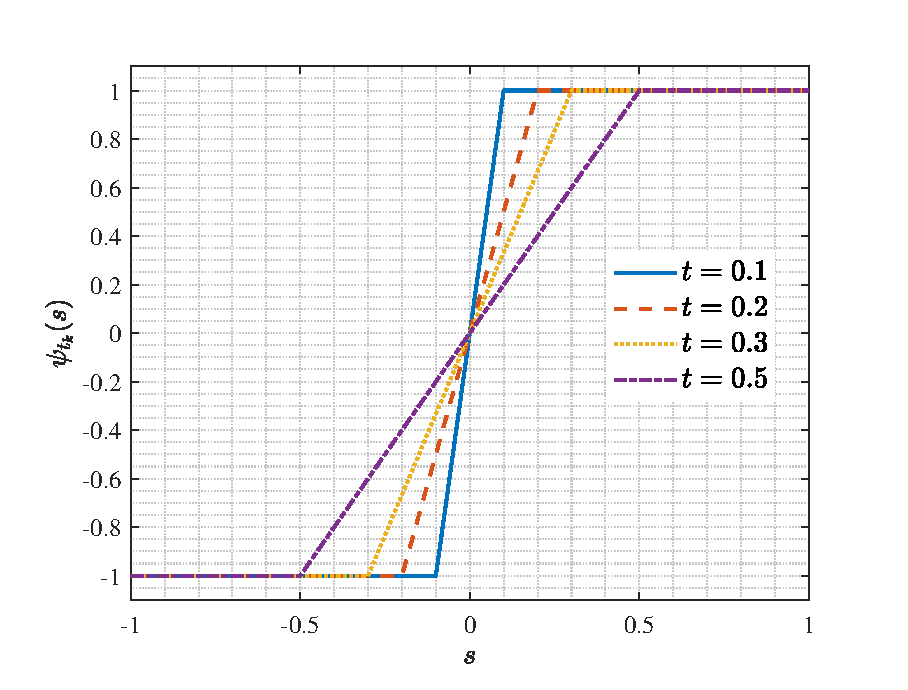
\includegraphics[width=.6\linewidth]{figures/soft_sign.eps}
    \caption{Hàm tuyến tính phân đoạn $\psi_{t_k}(s)$ được sử dụng trong DetNet.}
    \label{fig:soft_sign}
\end{figure}
Các tham số của việc học sẽ bao gồm 
\begin{equation}
\boldsymbol{\theta}=\left\{\mathbf{W}^1_{k}, \mathbf{b}^1_{k}, \mathbf{W}^2_{k}, \mathbf{b}^2_{k}, \mathbf{W}^3_{k}, \mathbf{b}^3_{ k}, \mathbf{t}_k\right\}_{k=1}^K
\end{equation}

Một hàm mất mát sẽ tổng hợp sai số từ kết quả đầu ra của tất cả các lớp để ước lượng sự hội tụ của mạng DetNet. Ngoài ra, vì các lỗi ước lượng từ DetNet còn phụ thuộc vào tính ngẫu nhiên của kênh truyền nên sẽ được chuẩn hoá bằng lỗi của bộ giải mã ZF. Hàm mất mát như dưới đây
\begin{equation}
\label{eq:lossdetnet}
    l(\mathbf{s} ; \hat{\mathbf{s}}(\mathbf{H}, \mathbf{x}))=\sum_{k=1}^K \log (k) \frac{\left\|\mathbf{s}-\hat{\mathbf{s}}_k\right\|^2}{\|\mathbf{s}-\tilde{\mathbf{s}}\|^2}
\end{equation}
với $\tilde{\mathbf{s}}$ là ước lượng của $\mathbf{s}$ thu được từ bộ giải mã ZF như trình bày trong mục~\ref{sec:zf}. Lưu ý rằng, do $\mathbf{H}$ là ma trận của các số thực nên phép chuyển vị liên hợp phức $(.)^H$ sẽ được chuyển thành chuyển vị $(.)^\top$.
\begin{equation}
    \tilde{\mathbf{s}}=\left(\mathbf{H}^\top \mathbf{H}\right)^{-1} \mathbf{H}^\top \mathbf{x}
\end{equation}

\section{Đề xuất mạng nơ-ron sâu ISDNN cho nhận dạng kênh truyền}

Trong phần này, giải thuật của bộ nhận dạng ISD đã được đề xuất trước đây sẽ được trình bày. Từ đó, một mạng nơ-ron sâu ISDNN được đề xuất dựa trên kỹ thuật mở rộng sâu cho giải thuật ISD trước đó.

\subsection{Bộ nhận dạng ISD cho kênh đường lên mMIMO}

Giải thuật gốc tại~\cite{Mandloi2017} đã đề xuất một bộ nhận dạng kênh truyền tuần tự lặp lại gọi tắt là ISD để đạt được hiệu suất của MMSE với độ phức tạp thấp. Trong đó, bộ nhận dạng MMSE đã được chứng minh~\cite{Rusek2013} có thể đạt được độ chính xác tiệm cận của MLE cho kênh đường lên cho các hệ mMIMO với $L/T \ge 10$.
\begin{equation}
    \hat{\mathbf{s}}_{MMSE}=\left(\mathbf{H}^\top \mathbf{H}+\frac{\sigma^2}{\mathbb{E}_\mathbf{s}} \mathbf{I}_{2T}\right)^{-1} \mathbf{H}^\top \mathbf{x}=\mathbf{P}^{-1} \mathbf{q}
\end{equation}
ký hiệu $\mathbf{G} = \mathbf{H}^\top \mathbf{H}$, $\mathbf{P} = \mathbf{H}^\top \mathbf{H}+\frac{\sigma^2}{\mathbb{E}_\mathbf{x}} \mathbf{I}_{2T}$, và $\mathbf{q} = \mathbf{H}^\top \mathbf{x}$. Các thành phần đường chéo (diagonal component) của ma trận $\mathbf{P}$ tạo thành ma trận $\mathbf{D}$. Lưu ý, độ phức tạp của việc nghịch đảo $\mathbf{P}$ là $\mathcal{O}(T^3)$, sẽ tăng nhanh khi $T$ lớn. 

Để đạt được hiệu năng cao hơn với ít số lần lặp lại,~\cite{Mandloi2017} đề xuất khởi tạo véc-tơ các ký hiệu đầu vào được ước lượng $\mathbf{s}$ như trên phương trình~(\ref{eq:sinit})~\cite{Gao2014} thay vì đặt tất cả bằng $0$.
\begin{equation}
\label{eq:sinit}
    \mathbf{s}_{in}=\mathbf{D}^{-1} \mathbf{q}=\left[s_0(1), s_0(2), \ldots, s_0(2T)\right]
\end{equation}

Từ véc-tơ tín hiệu thu, tín hiệu của ăng-ten/người dùng thứ $j$ thu được bằng cách loại bỏ tạp âm từ các ăng-ten/người dùng khác.
\begin{equation}
    \hat{\mathbf{x}}_j=\mathbf{x}-\sum_{t=1, t \neq j}^{2T} \mathbf{h}_t \hat{s}_k(t)
\end{equation}
với $\hat{\mathbf{x}}_j$ thu được, ký hiệu được gửi từ người dùng thứ $j$ được ước lượng như sau
\begin{equation}
\label{eq:supdate}
    \begin{aligned}
        \hat{s}_{k+1}(j) & =\frac{\mathbf{h}_j^\top}{\left\|\mathbf{h}_j\right\|^2} \hat{\mathbf{x}}_j \\ 
        & = \hat{s}_k(j)+\frac{1}{\mathbf{G}(j, j)}\left(\mathbf{q}(j)-\sum_{t=1}^{2T} \mathbf{G}(j, t) s_k(t)\right)
    \end{aligned}
\end{equation}
trong đó, $\mathbf{h}_j$ là cột thứ $j$ của ma trận $\mathbf{H}$, $\mathbf{G}(i, j)$ là phần tử thứ $(i, j)$ của ma trận $\mathbf{G}$, và $\mathbf{q}(j)$ là phần tử thứ $j$ của véc-tơ $\mathbf{q}$. Véc-tơ các ký hiệu ước lượng $\hat{\mathbf{s}}$ được cập nhật như trong thuật toán~\ref{alg:cap} của giải thuật ISD~\cite{Mandloi2017}. 
\begin{algorithm}[ht]
    \caption{Bộ nhận dạng Iterative Sequential~\cite{Mandloi2017}.}\label{alg:cap}
    \hspace*{\algorithmicindent} \textbf{Input: $\mathbf{x}, \mathbf{H}, L, T, K, \sigma^2, \mathbb{E}_\mathbf{s}$} \\
    \hspace*{\algorithmicindent} \textbf{Output: $\hat{\mathbf{s}}_{out} = \hat{\mathbf{s}}^{2T}_K$} 
    \begin{algorithmic}[1]
        \State $\mathbf{G} \leftarrow \mathbf{H}^\top \mathbf{H}$
        \State $\mathbf{A} \leftarrow \mathbf{G} + \frac{\sigma^2}{\mathbb{E}_\mathbf{x}} \mathbf{I}_{2T}$
        \State $\mathbf{s}_0 \leftarrow \mathbf{s}_{in} = \mathbf{D}^{-1} \mathbf{q}$ \\
        \For{ $k=0, k < K$}
            \For{ $j=1, j \le 2T$}
                \State $\hat{s}_k(j+1) \leftarrow \hat{s}_k(j)+\frac{1}{\mathbf{G}(j, j)}\left(\mathbf{q}(j)-\sum_{t=1}^{2T} \mathbf{G}(j, t) \hat{s}_k(t)\right)$ \\ 
                \State $\hat{\mathbf{s}}_{k+1}^j \leftarrow\left[\hat{s}_{k+1}(1),~\ldots, \hat{s}_{k+1}(j), \hat{s}_k(j+1),~\ldots, \hat{s}_k(2T)\right]$
                \State $j \leftarrow j + 1$
            \EndFor
            \State $k \leftarrow k + 1$
        \EndFor
    \end{algorithmic}
\end{algorithm}

Để chức minh giải thuật ISD là hiệu quả cho việc cước lượng kênh truyền, véc-tơ phần dư lỗi sẽ được sử dụng. Cụ thể, véc-tơ lỗi thu được sau khi khởi tạo với các giá trị $\mathbf{s}_0$ là
\begin{equation}
    \mathbf{e}_0 = \mathbf{x} - \mathbf{H} \mathbf{s}_0
\end{equation}
từ đó, véc-tơ phần dư lỗi sau khi cập nhật ký hiệu thứ $j$ tại vòng lặp/lớp thứ $k$ sẽ được biểu diễn như sau
\begin{equation}
    \mathbf{e}_k^{(j)}=\mathbf{x}-\mathbf{H} \hat{\mathbf{s}}_k^j
\end{equation}
thay $\mathbf{s}_k(j)$ bằng các biểu diễn hồi quy như trong giải thuật~\ref{alg:cap} thu được
\begin{equation}
\label{eq:eupdate}
\begin{aligned}
    \mathbf{e}_k^{(j)} & =\mathbf{x}-\mathbf{h}_j\left(\hat{s}_k(j-1)+\frac{1}{\mathbf{G}(j-1, j-1)}\left(\mathbf{q}(j-1)-\sum_{t=1}^{2T} \mathbf{G}(j-1, t) \hat{s}_k(t)\right)\right) \\
    & =\mathbf{x}-\mathbf{h}_j\left(\hat{s}_k(j-1)+\frac{1}{\mathbf{h}^\top_{j-1} \mathbf{h}_{j-1}}\left(\mathbf{h}_{j-1}^\top \mathbf{x}-\sum_{t=1}^{2T} \mathbf{G}(j-1, t) \hat{s}_k(t)\right)\right) \\
    & =\mathbf{e}_k^{(j-1)}-\mathbf{h}_{j} \frac{\mathbf{h}_j^\top}{\left\|\mathbf{h}_j\right\|^2} \mathbf{e}_k^{(j-1)}
    \end{aligned}
\end{equation}

Trong~\cite{Mandloi2017} đã chứng minh rằng $\left\|\mathbf{e}_k^{(j)}\right\|^2<\left\|\mathbf{e}_k^{(j-1)}\right\|^2$. Điều đó chỉ ra rằng mỗi khi ký hiệu thứ $j$ được cập nhật, véc-tơ lỗi sẽ được chiếu lên mặt phẳng `null' của cột thứ $j$ thuộc ma trận $\mathbf{H}$. Hay véc-tơ lỗi sẽ trực giao với $\mathbf{h}_j$, do đó $l_2-\operatorname{norm}$ bình phương của véc-tơ lỗi sẽ giảm sau mỗi lần ký hiệu $j$ được cập nhật cho đến khi $\mathbf{e}$ trực giao với không gian con kéo dài bởi cột của ma trận $\mathbf{H}$.

\subsection{Đề xuất mạng nơ-ron sâu ISDNN cho kênh đường lên mMIMO}

Từ giải thuật ISD được trình bày ở trên, theo hướng tiếp cận mở rộng sâu, một kiến trúc mạng nơ-ron sâu có tên ISDNN (Iterative sequential deep neural network) tương ứng được đề xuất. Đầu tiên, việc cập nhật các ký hiệu $\mathbf{s}$ được viết lại dưới dạng ma trận như sau
\begin{equation}
\hat{\mathbf{s}}_{k+1}=\hat{\mathbf{s}}_k+\mathbf{e}_{k+1}
\end{equation}
trong đó, $e_{k+1}$ là véc-tơ phần dư cũng được viết dưới dạng ma trận là
\begin{equation}
    \mathbf{e}_{k+1}=\mathbf{D}^{-1}\left(\mathbf{H}^\top \mathbf{x}-\mathbf{H}^\top \mathbf{H} \hat{\mathbf{s}}_k\right)
\end{equation}
Nhận thấy rằng, $\hat{\mathbf{s}}_{k+1}$ không chỉ chịu ảnh hưởng trực tiếp bởi $\mathbf{e}_{k+1}$ mà còn tất cả các véc-tơ phần dư trước đó $\mathbf{e}_{k}, \mathbf{e}_{k-1},~\ldots, \mathbf{e}_{1}$ như biểu diễn ở công thức (\ref{eq:eupdate}). Do vậy, để đạt được hiệu quả cao hơn trong việc loại bỏ tạp âm từ các người dùng khác, chúng tôi đề xuất thêm vào các tham số học $\alpha^1_k$ vào mỗi lớp (layer) của mạng nơ-ron.
\begin{equation}
\label{eq:supdate1}
\hat{\mathbf{s}}_{k+1}=\hat{\mathbf{s}}_k+\mathbf{e}_{k+1}+\alpha_k^{1} \mathbf{e}_k+\alpha_{k-1}^{1} \mathbf{e}_{k-1}+\cdots+\alpha_1^{1} \mathbf{e}_1
\end{equation}

Tuy nhiên, mối tương quan giữa các véc-tơ phần dư liền kề là lớn nhất, nên trong mạng ISDNN chỉ xem xét ảnh hưởng của $\mathbf{e}_k$ ở lớp thứ $k$ đề đơn giản hoá mô hình. Phương trình (\ref{eq:supdate1}) trở thành 
\begin{equation}
\mu_{k}=\hat{\mathbf{s}}_k+\mathbf{e}_{k+1}+\alpha_k^1 \mathbf{e}_k
\end{equation}

Để đảm bảo $\hat{\mathbf{s}}_{k+1}$ sẽ hội tụ, tác giả đề xuất thêm một tham số học $\alpha^2_k$ với $\sum_{i=k}^{k+1} \alpha_i^{2} \hat{\mathbf{s}}_i$ with $\sum_{i=k}^{k+1} \alpha_i^{2}=1$ tại mỗi lớp như sau
\begin{equation}
\hat{\mathbf{s}}_{k+1}=\left(1-\alpha_k^2\right) \mu_k + \alpha_k^2 \hat{\mathbf{s}}_k
\end{equation}

Ngoài ra, để đạt được độ chính xác cao hơn ở các loại điều chế bậc cao như (16-QAM, 64-QAM,~\ldots), véc-tơ phần dư sẽ được điều chỉnh linh hoạt hơn bằng cách thêm hai lớp nhỏ hơn vào kiến trúc mạng ISDNN để cập nhật $\mathbf{e}_k$ trước khi nhân với $\alpha^1_k$.
\begin{equation}
\mathbf{e}_k \leftarrow \mathbf{W}^2_{k}\left(\mathbf{W}^1_{k} \mathbf{e}_k+\mathbf{b}^1_{k}\right)+\mathbf{b}^2_{k}
\end{equation}

Kiến trúc cuối cùng của mạng ISDNN được đề xuất trong luận văn như trên hình~\ref{fig:ISD}. So với giải thuật ISD được đề xuất trước đó, mạng nơ-ron sâu ISDNN được đề xuất có sự cải tiến bằng việc (i) thêm véc-tơ phần dư của lớp trước đó và tham số học $\alpha^1$ để ước lượng $\hat{\mathbf{s}}$, (ii) tham số học $\alpha^2$ được thêm vào để đảm bảo sự hội tụ của việc học, (iii) véc-tơ phần dư được đưa qua hai lớp mạng để có được tính linh hoạt cho các loại điều chế bậc cao.
\begin{figure}[ht]
    \centering
    \begin{tikzpicture}
        \node (B11) [field6, fill=red!10!white] at (0, 0) {$\mathbf{e}_0$};
        \node (B21) [below=10mm of B11, field6, fill=red!10!white] {$\mathbf{s}_0$};
        \node (B31) [below=10mm of B21, field6, fill=red!10!white] {$\mathbf{H}^\top \mathbf{H}$};
        \node (B41) [below=10mm of B31, field6, fill=red!10!white] {$\mathbf{H}^\top \mathbf{x}$};
        \node (B51) [below=10mm of B41, field6, fill=red!10!white] {$\mathbf{D}^{-1}$};

        \node (B12) [right=5mm of B11, circle, fill=blue!10!white, draw=black] {$\times$};
        \node (B13) [right=5mm of B12, circle, fill=blue!10!white, draw=black] {$+$};
        \node (B14) [right=5mm of B13, circle, fill=blue!10!white, draw=black] {$\times$};
        \node (B15) [right=5mm of B14, circle, fill=blue!10!white, draw=black] {$+$};
        \node (B16) [right=5mm of B15, circle, fill=blue!10!white, draw=black] {$\times$};
        \node (B17) [right=18mm of B16, field8, fill=green!10!white, draw=black] {$\alpha^2_0$};
        \node (B18) [right=5mm of B17, circle, fill=blue!10!white, draw=black] {$\times$};

        \node (B61) [below=4mm of B12, field8, fill=green!10!white, draw=black] {$\mathbf{W}^1_{0}$};
        \node (B62) [below=4mm of B13, field8, fill=green!10!white, draw=black] {$\mathbf{b}^1_{0}$};
        \node (B63) [below=4mm of B14, field8, fill=green!10!white, draw=black] {$\mathbf{W}^2_{0}$};
        \node (B64) [below=4mm of B15, field8, fill=green!10!white, draw=black] {$\mathbf{b}^2_{0}$};
        \node (B65) [below=4mm of B16, field8, fill=green!10!white, draw=black] {$\alpha^1_0$};

        \node (B22) [right=75mm of B21, circle, fill=blue!10!white, draw=black] {$+$};
        \node (B23) [below=12mm of B18, circle, fill=blue!10!white, draw=black] {$+$};
        \node (B24) [right=5mm of B23, circle, fill=blue!10!white, draw=black] {$\rho$};

        \node (B25) [below=4mm of B23, circle, fill=blue!10!white, draw=black] {$\times$};
        \node (B26) [below=4mm of B25, field8, fill=green!10!white, draw=black] {$1 - \alpha^2_0$};

        \node (B32) [right=5mm of B31, circle, fill=blue!10!white, draw=black] {$\times$};
        \node (B42) [right=5mm of B41, circle, fill=blue!10!white, draw=black] {$-$};
        \node (B52) [right=5mm of B51, circle, fill=blue!10!white, draw=black] {$\times$};

        \node (Phi1) [right=123mm of B21, field6, fill=red!10!white] {$\hat{\mathbf{s}}_1$};
        \node (V1) [right=123mm of B51, field6, fill=red!10!white] {$\mathbf{e}_{1}$};

        \draw[arrow] (B11) -- (B12);
        \draw[arrow] (B12) -- (B13);
        \draw[arrow] (B13) -- (B14);
        \draw[arrow] (B14) -- (B15);
        \draw[arrow] (B15) -- (B16);
        \draw[arrow] (B17) -- (B18);
        
        \draw[arrow] (B61) -- (B12);
        \draw[arrow] (B62) -- (B13);
        \draw[arrow] (B63) -- (B14);
        \draw[arrow] (B64) -- (B15);
        \draw[arrow] (B65) -- (B16);

        \draw[arrow] (B21) -- (B22);
        \draw[arrow] (B31) -- (B32);
        \draw[arrow] (B41) -- (B42);
        \draw[arrow] (B51) -- (B52);
        \draw[arrow] (B52) -- (V1);

        \draw[arrow] (B18) -- (B23);
        \draw[arrow] (B23) -- (B24);
        \draw[arrow] (B24) -- (Phi1);

        \draw[arrow] (B16) -| (B22);
        \draw[arrow] (B25) -- (B23);
        \draw[arrow] (B26) -- (B25);
        \draw[line] (B22) -- ([xshift=3mm]B22.east);
        \draw[arrow] ([xshift=3mm]B22.east) |- (B25);
        \draw[line] (V1) -- ([yshift=15mm]V1.north);
        \draw[arrow] ([yshift=15mm]V1.north) -| (B22);

        \draw[arrow] (B21) -| (B32);
        \draw[arrow] (B32) -- (B42);
        \draw[arrow] (B42) -- (B52);

        \draw[line] (B21) -| ([xshift=-3mm, yshift=28mm]B21.west);
        \draw[arrow] ([xshift=-3mm, yshift=28mm]B21.west) -| (B18);

        \draw[arrow] (Phi1) -- ([xshift=3mm]Phi1.east);
        \draw[arrow] (V1) -- ([xshift=3mm]V1.east);

        % Legends
        \node[rectangle, draw=black, dashed, fill=black!5!white, minimum width=100mm, minimum height=35mm] at (70mm, -105mm) {};

        \node (B51) [field6, fill=red!10!white] at (37mm, -97mm) {Giá trị \\đầu vào/đầu ra};

        \node (B61) [below=4mm of B51, field8, fill=green!10!white, draw=black] {Giá trị học};

        \node (B52) [right=7mm of B51, circle, fill=blue!10!white, draw=black] {$\times$};
        \draw[arrow] (B52) -- ([xshift=3mm]B52.east) node [pos=0, right=3mm] {Nhân};

        \node (B53) [below=7mm of B52, circle, fill=blue!10!white, draw=black] {$+$};
        \draw[arrow] (B53) -- ([xshift=3mm]B53.east) node [pos=0, right=3mm] {Cộng};

        \node (B54) [right=20mm of B52, circle, fill=blue!10!white, draw=black] {$\rho$};
        \draw[arrow] (B54) -- ([xshift=10mm]B54.east) node [pos=0, right=10mm, above, label={below}:{tuyến tính}] {Toán tử};

        \node (B55) [right=20mm of B53, circle, fill=blue!10!white, draw=black] {$-$};
        \draw[arrow] (B55) -- ([xshift=3mm]B55.east) node [pos=0, right=3mm] {Trừ};
    \end{tikzpicture}
    \caption{Kiến trúc của lớp đầu tiên trong mô hình mạng ISD đề xuất.}
    \label{fig:ISD}
\end{figure}

Các tham số khởi tạo của mạng ISDNN được đề xuất như sau để nhanh chóng đạt được sự hội tụ~\cite{Narasimhan2014}: $\mathbf{s}_0 = \mathbf{D}^{-1}\mathbf{q}$; $\alpha^1_0$ được chọn ngẫu nhiên tiệm cận $0$ ($\alpha^1_0 \approx 0$); $\alpha^2_0 = 0$,$5$. Do các đầu vào cho lớp tiếp theo $\hat{\mathbf{s}}_{k+1}$ cần được ánh xạ về khoảng giá trị $[-1.0 \;\; 1.0]$, một hàm kích hoạt tuyến tính (activation function) sẽ được sử dụng. Trong DL, có nhiều hàm kích hoạt được sử dụng rộng rãi như ReLu, Tanh, Sigmoid,~\ldots như được biểu diễn trên hình~\ref{fig:tanh}. Cụ thể, trong ISDNN, tác giả lựa chọn sử dụng hàm Tanh có biểu diễn toán học như sau
\begin{equation}
    \operatorname{Tanh}(s) = \frac{e^s - e^{-s}}{e^s + e^{-s}}
\end{equation}
\begin{figure}[ht]
    \centering
    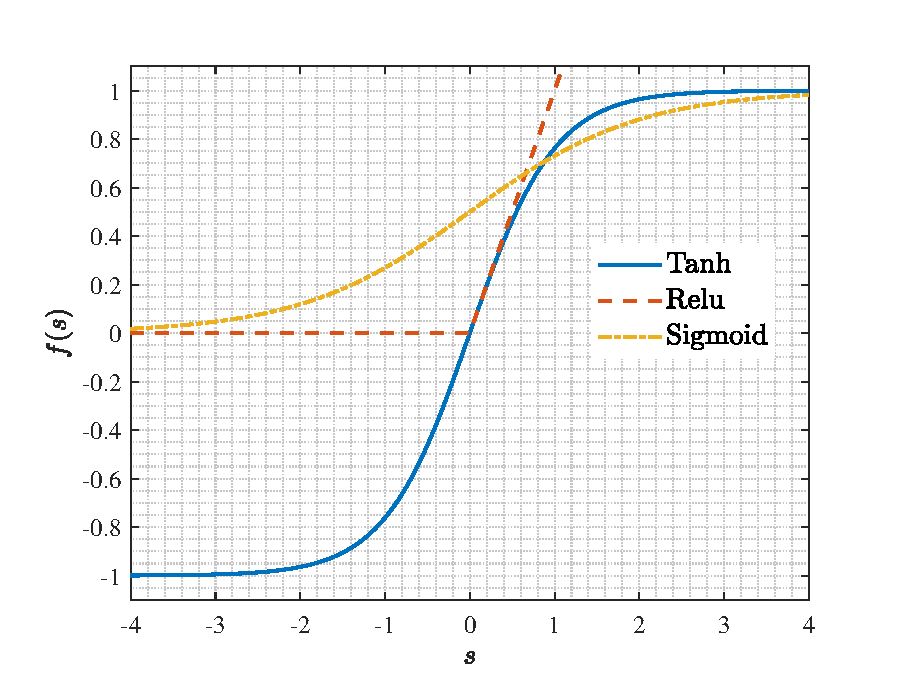
\includegraphics[width=.6\linewidth]{figures/tanh.eps}
    \caption{Minh hoạ một số hàm kích hoạt được dùng trong mô hình đề xuất.}
    \label{fig:tanh}
\end{figure}

Các tham số của việc học sẽ bao gồm 
\begin{equation}
\boldsymbol{\theta}=\left\{\mathbf{W}^1_{k}, \mathbf{b}^1_{k}, \mathbf{W}^2_{k}, \mathbf{b}^2_{k}, \alpha^1_k, \alpha^2_k \right\}_{k=1}^K
\end{equation}

Một hàm mất mát cũng được định nghĩa như trên phương trình (\ref{eq:lossdetnet}) để biểu diễn sự hội tụ của mô hình học ISDNN.

\section{Mô phỏng và đánh giá}

\subsection{Tạo bộ dữ liệu}

\begin{table}
    \centering
    \caption{Các tham số mô phỏng hệ thống truyền thông không dây của mạng ISD được đề xuất.}
    \label{tab:simu_param}
    \begin{tabular}{p{8cm}|p{6cm}} 
    \hline
    \hline
    \multicolumn{1}{c|}{\textbf{Thông số mô phỏng}} & \multicolumn{1}{c} {\textbf{Giá trị}} \\ 
    \hline
    Kích thước hệ thống m-MIMO & $T = 8, L =64$ \\ 
    \hline
    Loại điều chế & 16-QAM\\
    \hline
    Các mức $\operatorname{SNR}$ của dataset  & $[0, 5, 10, 15, 20]$~dB \\ 
    \hline
    Số mẫu đào tạo & 50.000 \\ 
    \hline
    Số mẫu thử nghiệm & 10.000 \\ 
    \hline
    Bộ tối ưu & ADAM \\ 
    \hline
    Giá trị khởi tạo của tỷ lệ học & $\delta = 0$,$0001$ \\ 
    \hline
    Số vòng lặp đào tạo & 200.000 \\
    \hline
    \end{tabular}
\end{table}

\subsection{Đào tạo và đánh giá mô hình đề xuất}

\begin{table}[ht]
    \centering
    \caption{So sánh độ phức tạp của các thuật toán nhận dạng kênh truyền.}
    \label{tab:computational}
    \begin{tabular}{|l|c|c|}
    \hline
    \multicolumn{1}{|c|}{Detector} & Computational complexity & Trainable parameters \\ \hline
    ZF & $\mathcal{O}$ ($NK^3$) &  \\ \hline
    MMSE & $\mathcal{O}$ ($NK^3$) &  \\ \hline
    MLE & $\mathcal{O}$ ($NK^3$) &  \\ \hline
    DetNet~\cite{Samuel2019} & $\mathcal{O}$ ($NK^2$) & 249600 \\ \hline
    Proposed ISD & $\mathcal{O}$ ($NK^2$) & 12 \\ \hline
    \end{tabular}
\end{table}

\section{Kết luận chương}